\documentclass[../document.tex]{subfiles}
\begin{document}
\subsection{Robustness}
To test is robustness we will create custom patches with different features, walls/bumps/ramps, and test the model prediction against the real robot advancement obtained from the simulator. We always used a \emph{threhold} of $20$cm and a time window of two seconds. 
\subsubsection{Wall in front of Krock}
The easiest test we can perform is to place a wall in front of \emph{Krock}. If we place the wall at different distance from the Krock's head we should reach a point where, moving the wall towards the end of the patch, the model should yield traversable even if the wall itself is tall. Why? Because the robot will be able to traverse more than the threshold before beeing stopped by the wall.


We create different patches by first placing the wall exactly in front of the robot and then move it $1$cm at the time towards the end. The following images shows the patches with the wall starting from a wall at $1$cm from the robot till the end of the patch.
\begin{figure}[H]
    \centering
    \begin{subfigure}[b]{0.065\textwidth}
    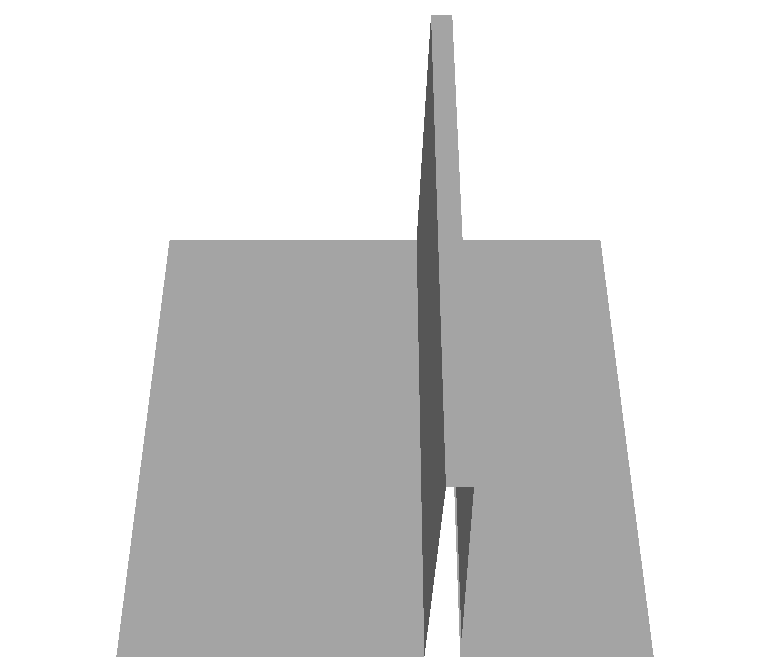
\includegraphics[width=\linewidth]{../img/5/custom_patches/walls_front/all/55-3d.png}
    \end{subfigure}
    \begin{subfigure}[b]{0.065\textwidth}
    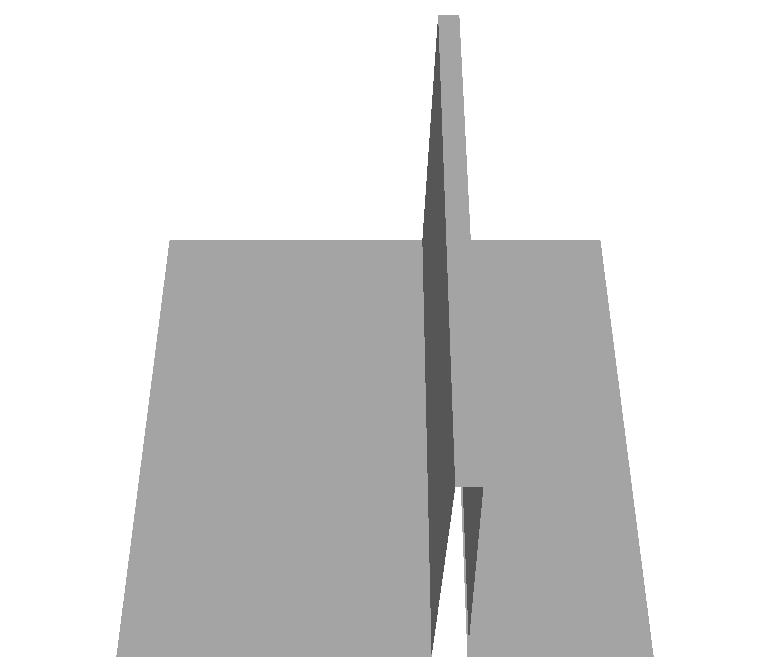
\includegraphics[width=\linewidth]{../img/5/custom_patches/walls_front/all/54-3d.png}
    \end{subfigure}
    \begin{subfigure}[b]{0.065\textwidth}
    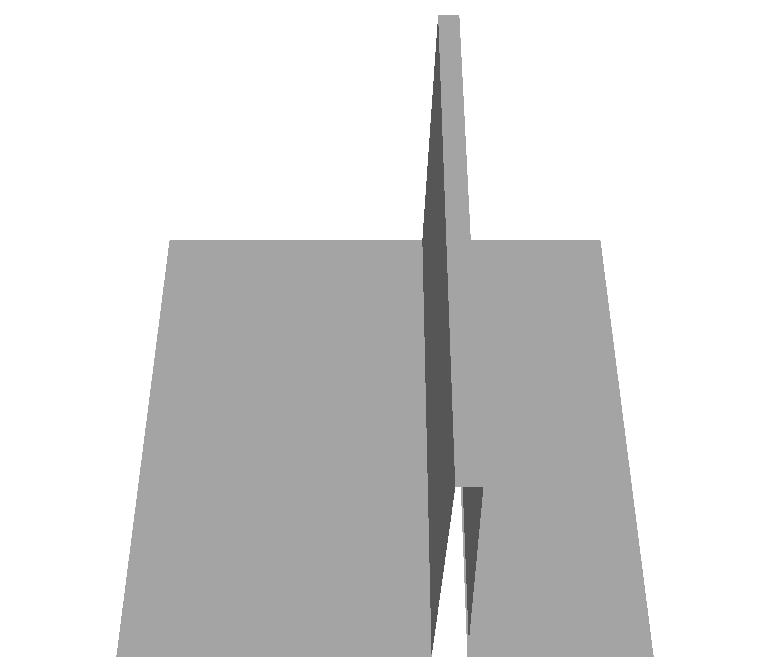
\includegraphics[width=\linewidth]{../img/5/custom_patches/walls_front/all/53-3d.png}
    \end{subfigure}
    \begin{subfigure}[b]{0.065\textwidth}
    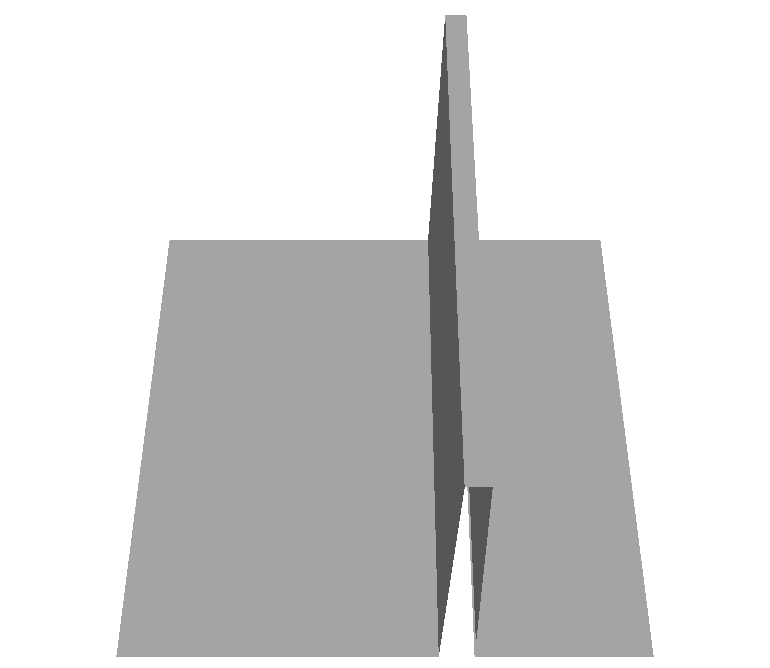
\includegraphics[width=\linewidth]{../img/5/custom_patches/walls_front/all/52-3d.png}
    \end{subfigure}
    \begin{subfigure}[b]{0.065\textwidth}
    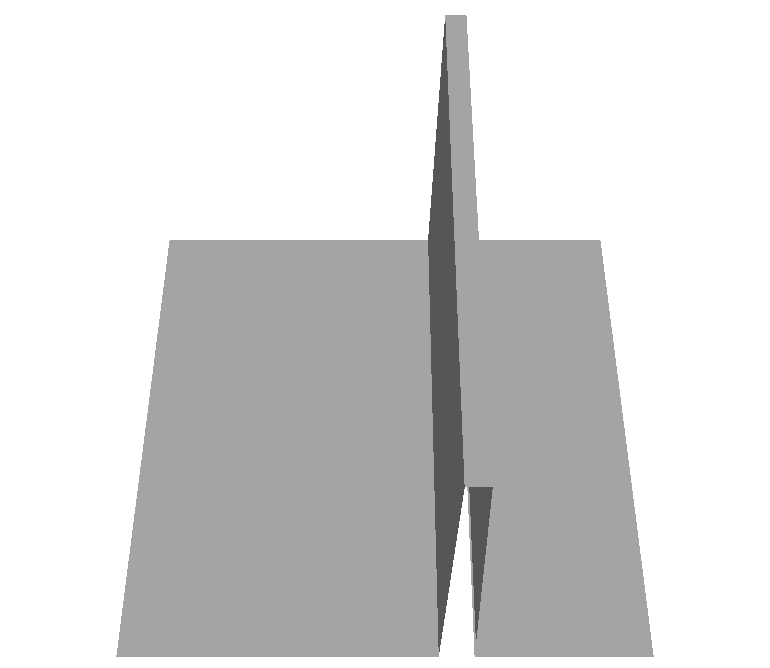
\includegraphics[width=\linewidth]{../img/5/custom_patches/walls_front/all/51-3d.png}
    \end{subfigure}
    \begin{subfigure}[b]{0.065\textwidth}
    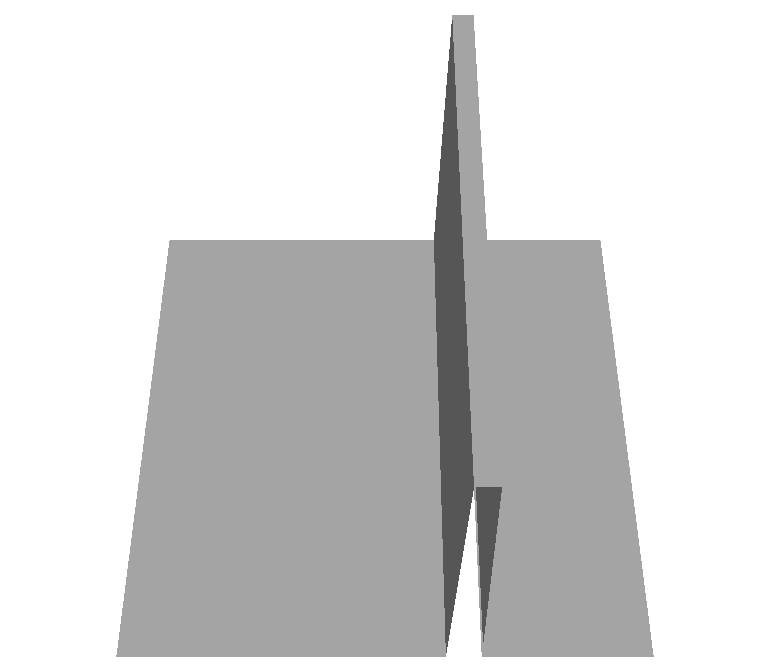
\includegraphics[width=\linewidth]{../img/5/custom_patches/walls_front/all/50-3d.png}
    \end{subfigure}
    \begin{subfigure}[b]{0.065\textwidth}
    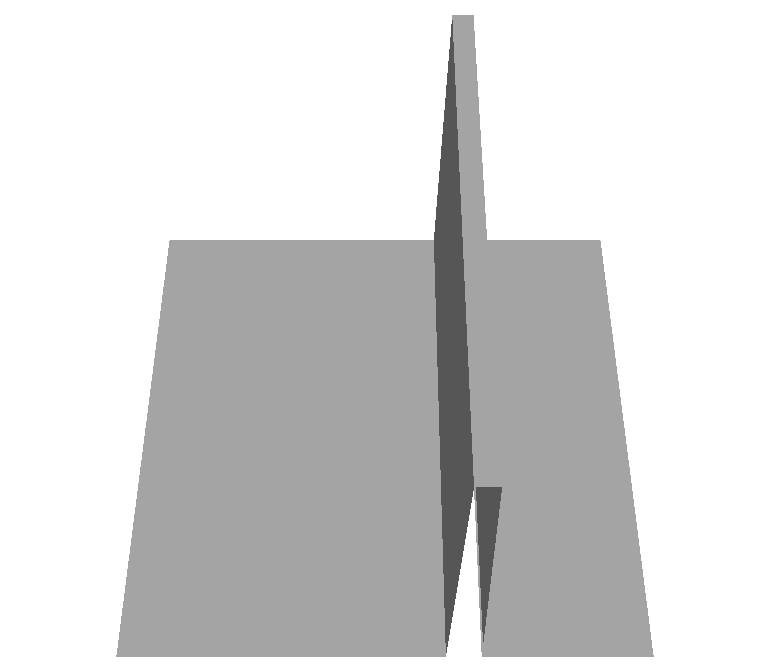
\includegraphics[width=\linewidth]{../img/5/custom_patches/walls_front/all/49-3d.png}
    \end{subfigure}
    \begin{subfigure}[b]{0.065\textwidth}
    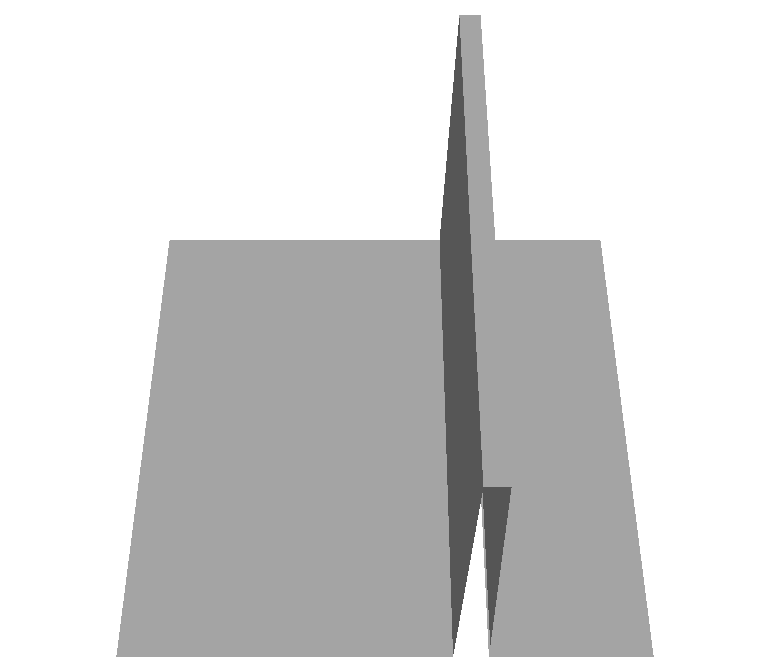
\includegraphics[width=\linewidth]{../img/5/custom_patches/walls_front/all/48-3d.png}
    \end{subfigure}
    \begin{subfigure}[b]{0.065\textwidth}
    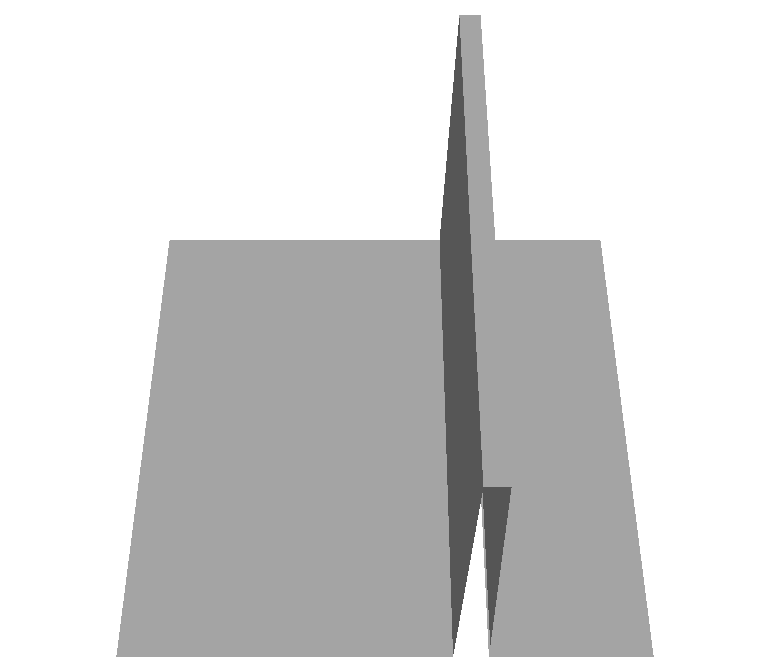
\includegraphics[width=\linewidth]{../img/5/custom_patches/walls_front/all/47-3d.png}
    \end{subfigure}
    \begin{subfigure}[b]{0.065\textwidth}
    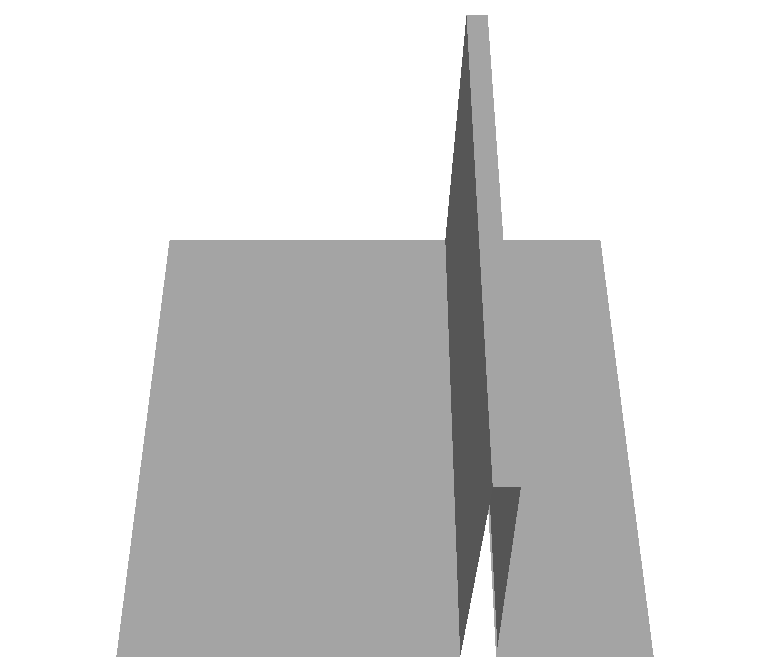
\includegraphics[width=\linewidth]{../img/5/custom_patches/walls_front/all/46-3d.png}
    \end{subfigure}
    \begin{subfigure}[b]{0.065\textwidth}
    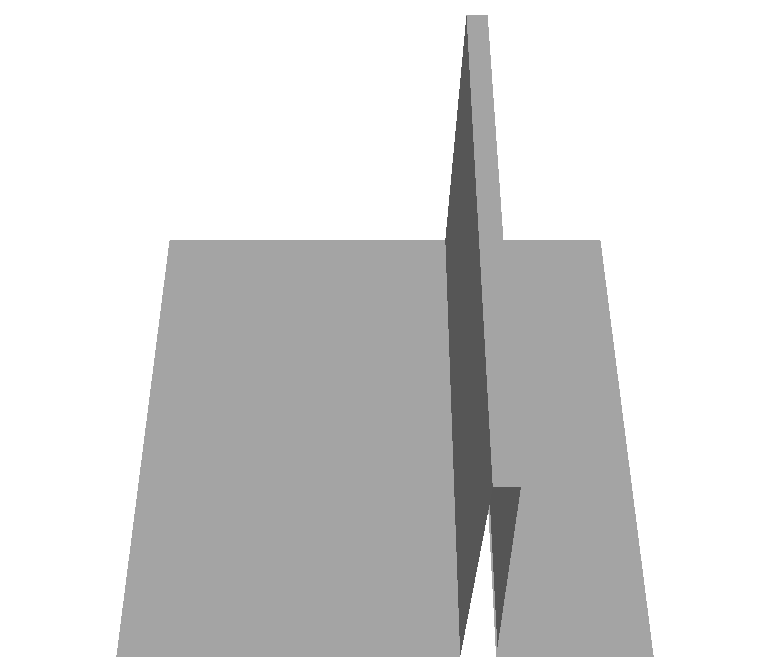
\includegraphics[width=\linewidth]{../img/5/custom_patches/walls_front/all/45-3d.png}
    \end{subfigure}
    \begin{subfigure}[b]{0.065\textwidth}
    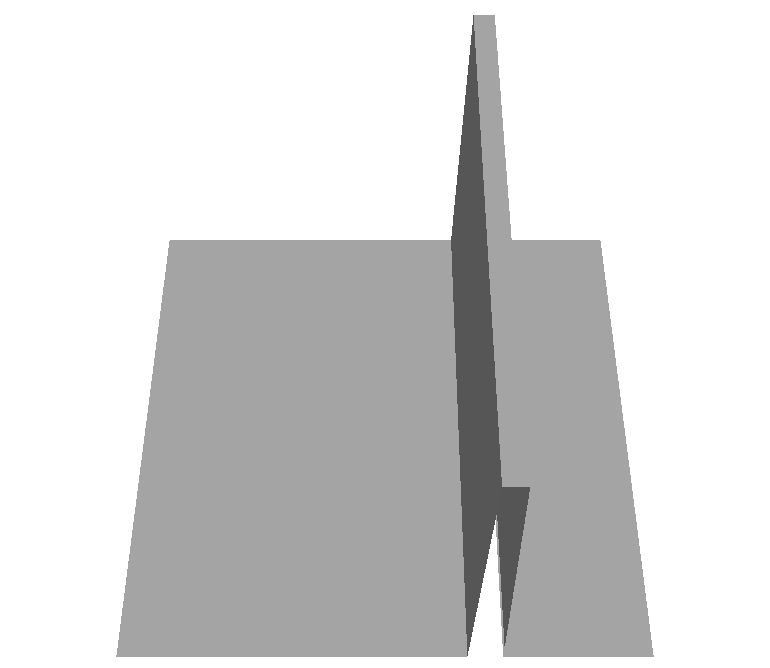
\includegraphics[width=\linewidth]{../img/5/custom_patches/walls_front/all/44-3d.png}
    \end{subfigure}
    \begin{subfigure}[b]{0.065\textwidth}
    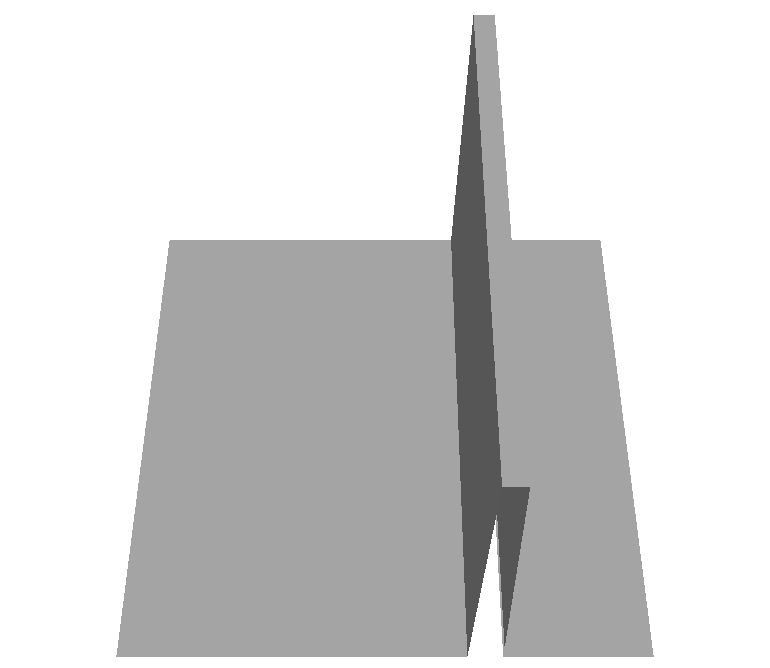
\includegraphics[width=\linewidth]{../img/5/custom_patches/walls_front/all/43-3d.png}
    \end{subfigure}
    \begin{subfigure}[b]{0.065\textwidth}
    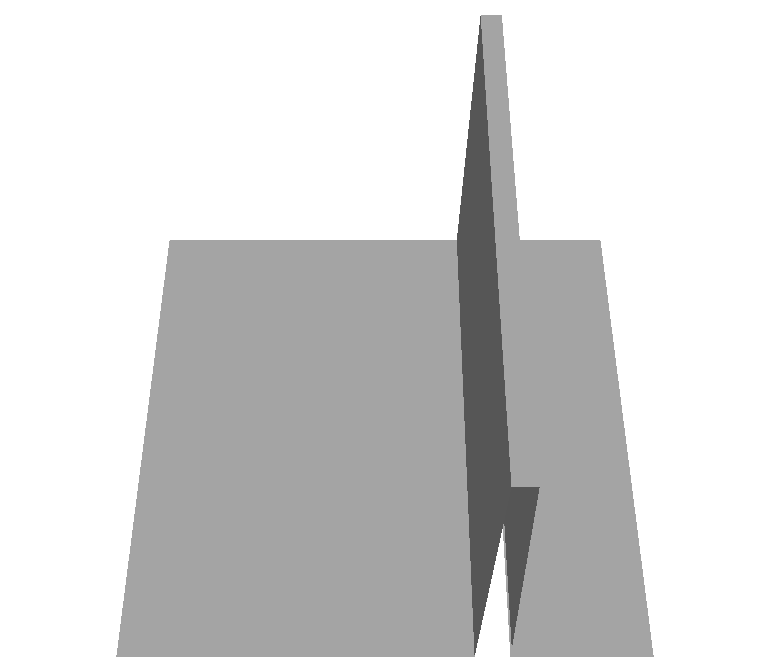
\includegraphics[width=\linewidth]{../img/5/custom_patches/walls_front/all/42-3d.png}
    \end{subfigure}
    \begin{subfigure}[b]{0.065\textwidth}
    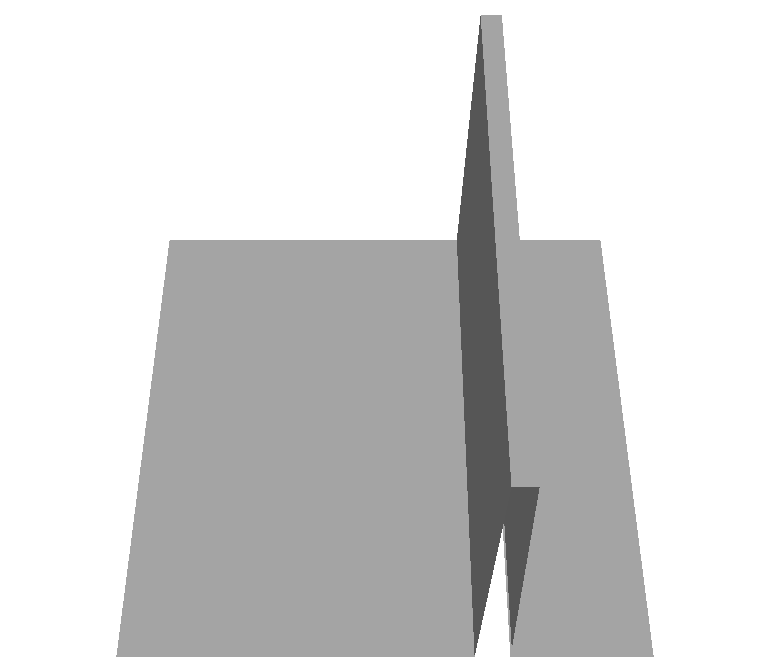
\includegraphics[width=\linewidth]{../img/5/custom_patches/walls_front/all/41-3d.png}
    \end{subfigure}
    \begin{subfigure}[b]{0.065\textwidth}
    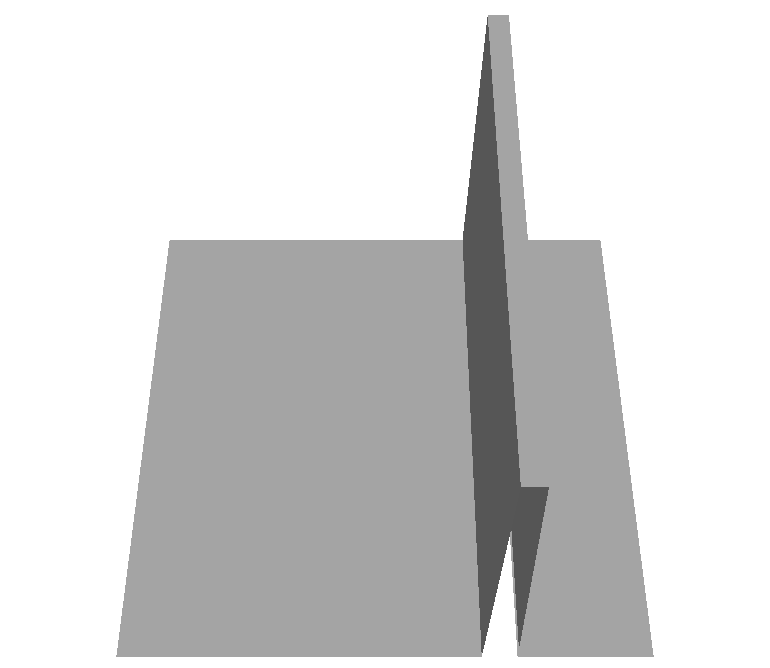
\includegraphics[width=\linewidth]{../img/5/custom_patches/walls_front/all/40-3d.png}
    \end{subfigure}
    \begin{subfigure}[b]{0.065\textwidth}
    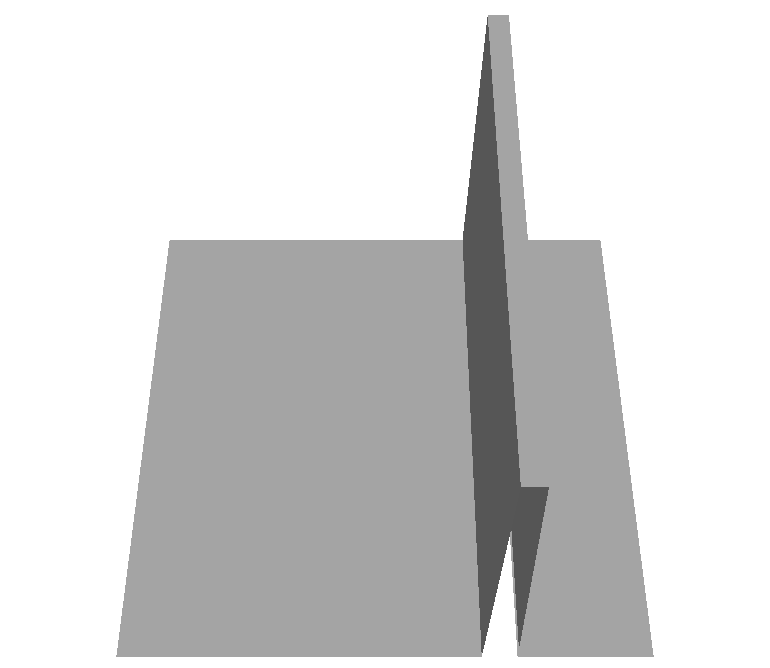
\includegraphics[width=\linewidth]{../img/5/custom_patches/walls_front/all/39-3d.png}
    \end{subfigure}
    \begin{subfigure}[b]{0.065\textwidth}
    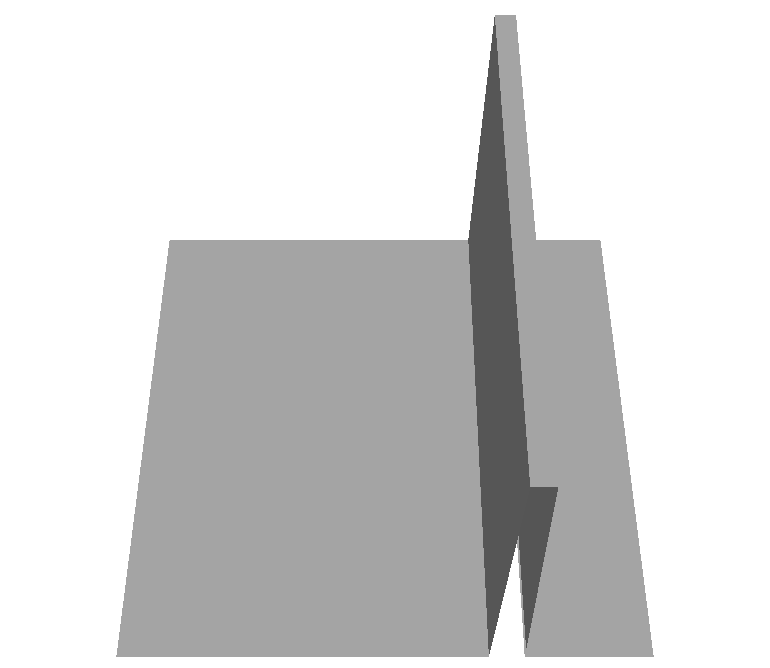
\includegraphics[width=\linewidth]{../img/5/custom_patches/walls_front/all/38-3d.png}
    \end{subfigure}
    \begin{subfigure}[b]{0.065\textwidth}
    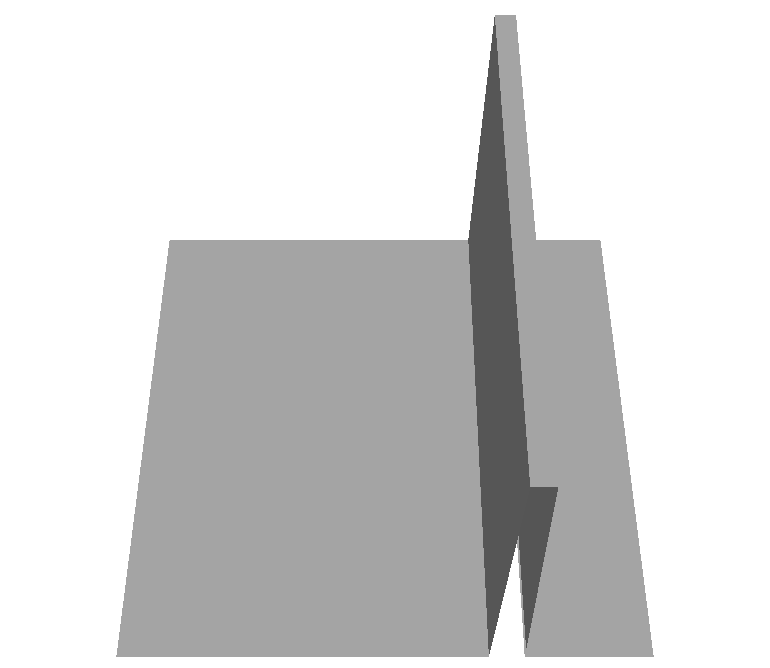
\includegraphics[width=\linewidth]{../img/5/custom_patches/walls_front/all/37-3d.png}
    \end{subfigure}
    \begin{subfigure}[b]{0.065\textwidth}
    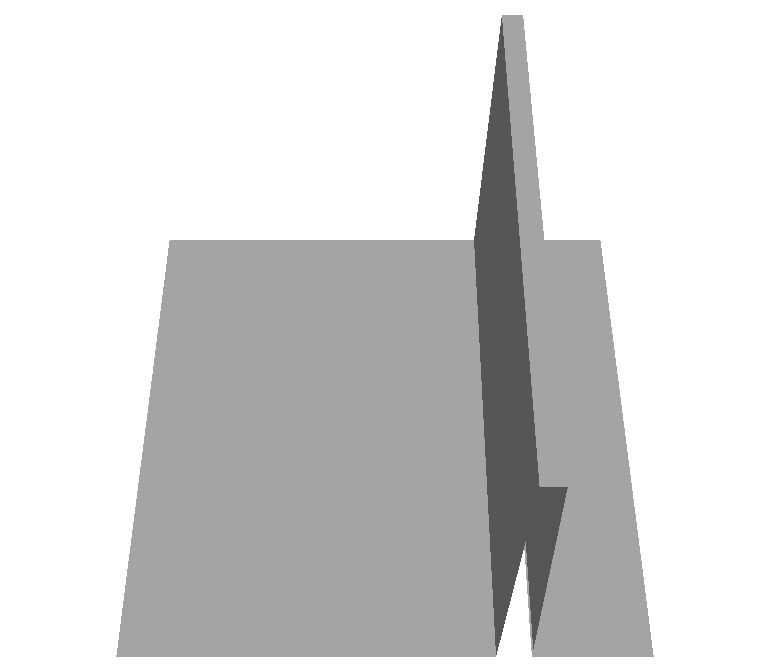
\includegraphics[width=\linewidth]{../img/5/custom_patches/walls_front/all/36-3d.png}
    \end{subfigure}
    \begin{subfigure}[b]{0.065\textwidth}
    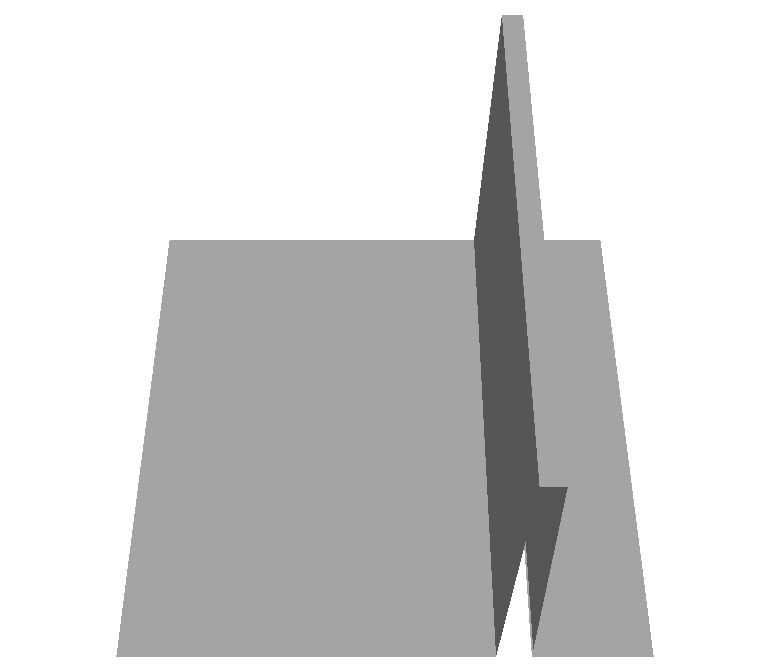
\includegraphics[width=\linewidth]{../img/5/custom_patches/walls_front/all/35-3d.png}
    \end{subfigure}
    \begin{subfigure}[b]{0.065\textwidth}
    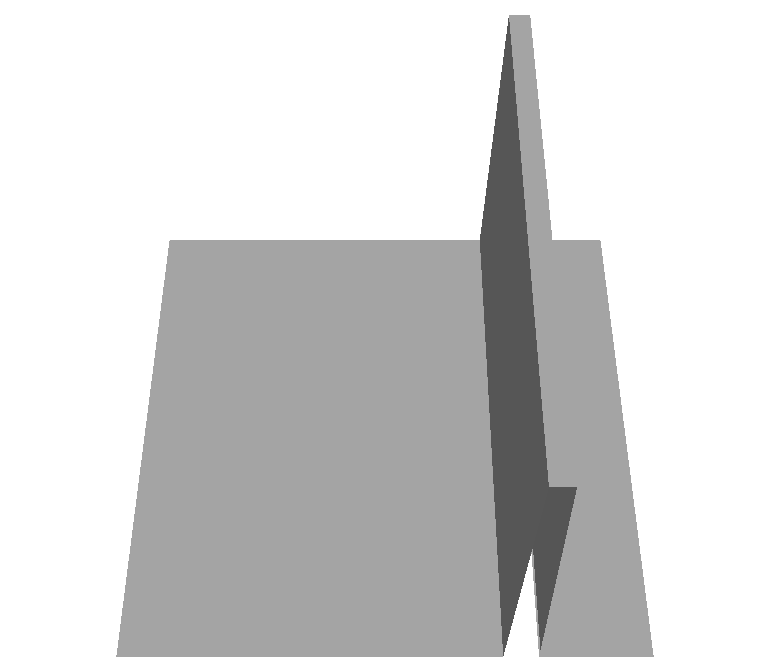
\includegraphics[width=\linewidth]{../img/5/custom_patches/walls_front/all/34-3d.png}
    \end{subfigure}
    \begin{subfigure}[b]{0.065\textwidth}
    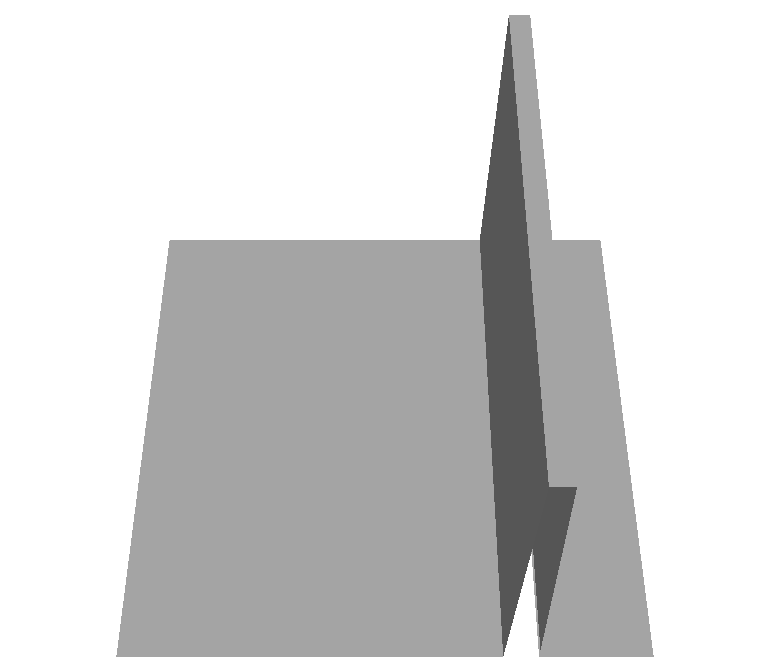
\includegraphics[width=\linewidth]{../img/5/custom_patches/walls_front/all/33-3d.png}
    \end{subfigure}
    \begin{subfigure}[b]{0.065\textwidth}
    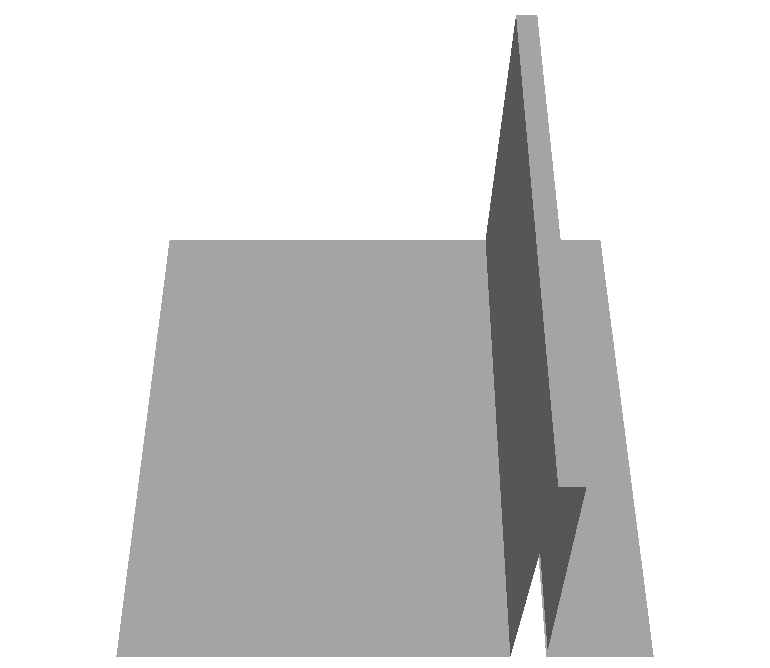
\includegraphics[width=\linewidth]{../img/5/custom_patches/walls_front/all/32-3d.png}
    \end{subfigure}
    \begin{subfigure}[b]{0.065\textwidth}
    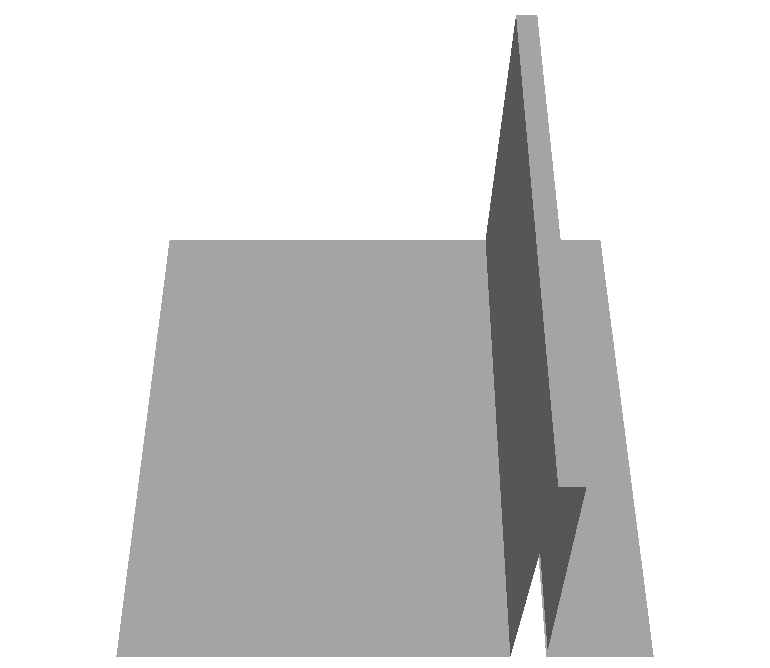
\includegraphics[width=\linewidth]{../img/5/custom_patches/walls_front/all/31-3d.png}
    \end{subfigure}
    \begin{subfigure}[b]{0.065\textwidth}
    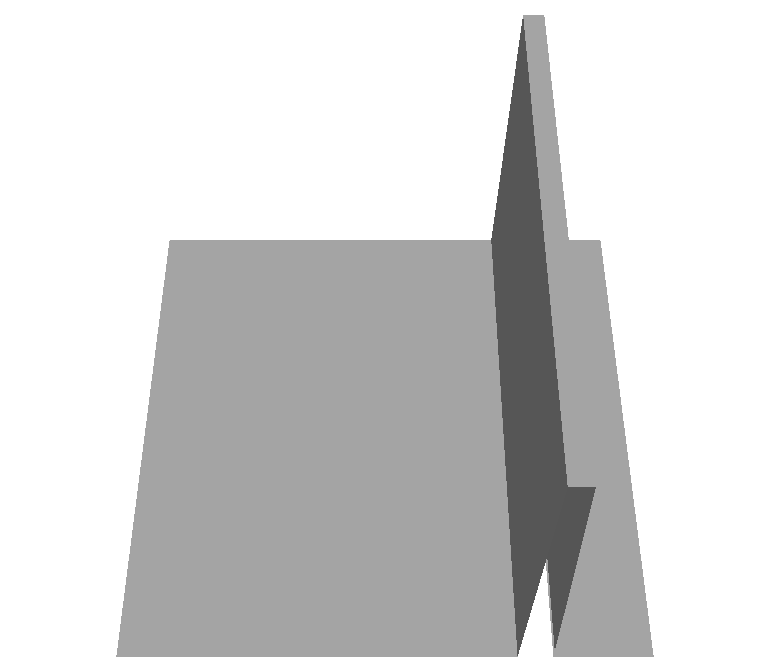
\includegraphics[width=\linewidth]{../img/5/custom_patches/walls_front/all/30-3d.png}
    \end{subfigure}
    \begin{subfigure}[b]{0.065\textwidth}
    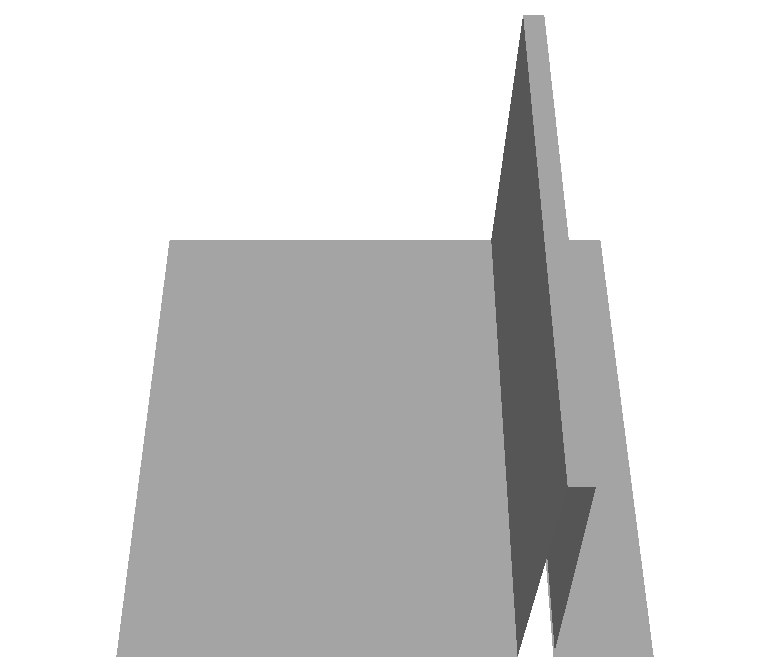
\includegraphics[width=\linewidth]{../img/5/custom_patches/walls_front/all/29-3d.png}
    \end{subfigure}
    \begin{subfigure}[b]{0.065\textwidth}
    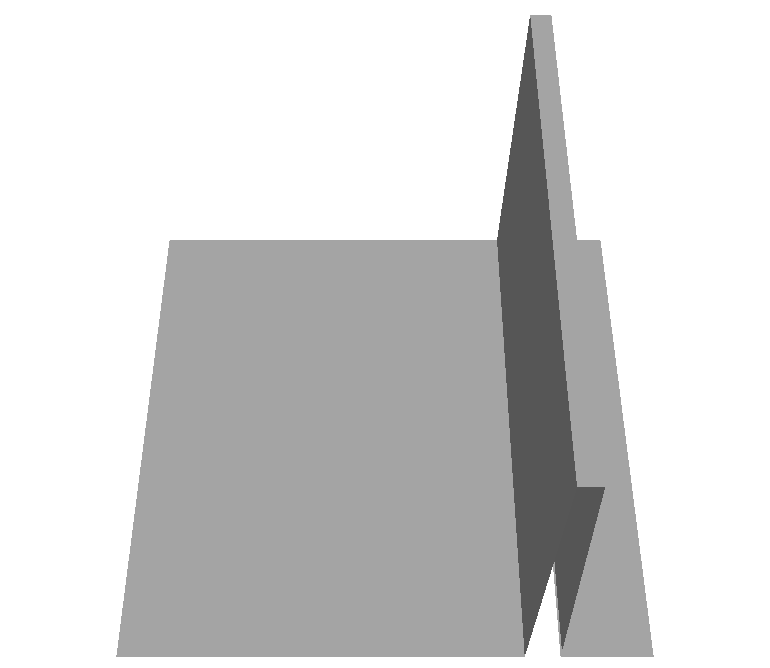
\includegraphics[width=\linewidth]{../img/5/custom_patches/walls_front/all/28-3d.png}
    \end{subfigure}
    \begin{subfigure}[b]{0.065\textwidth}
    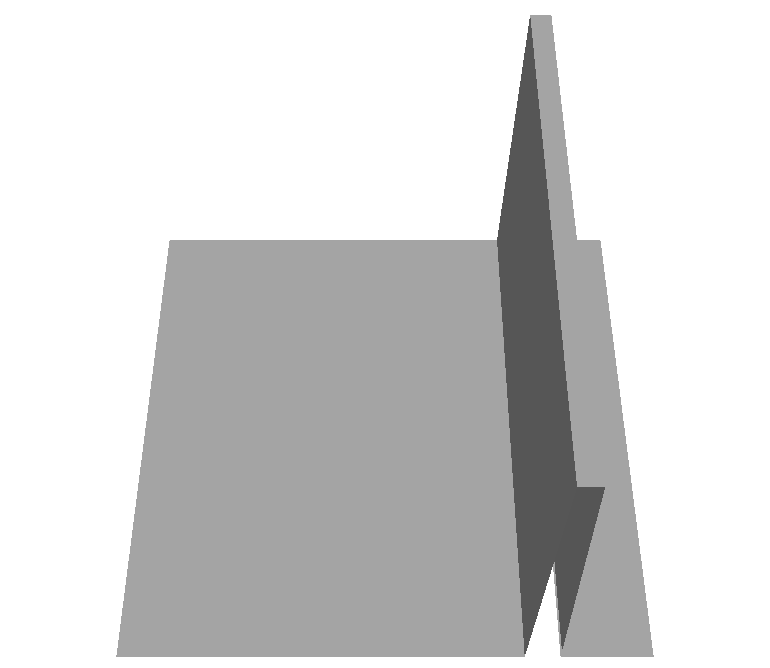
\includegraphics[width=\linewidth]{../img/5/custom_patches/walls_front/all/27-3d.png}
    \end{subfigure}
    \begin{subfigure}[b]{0.065\textwidth}
    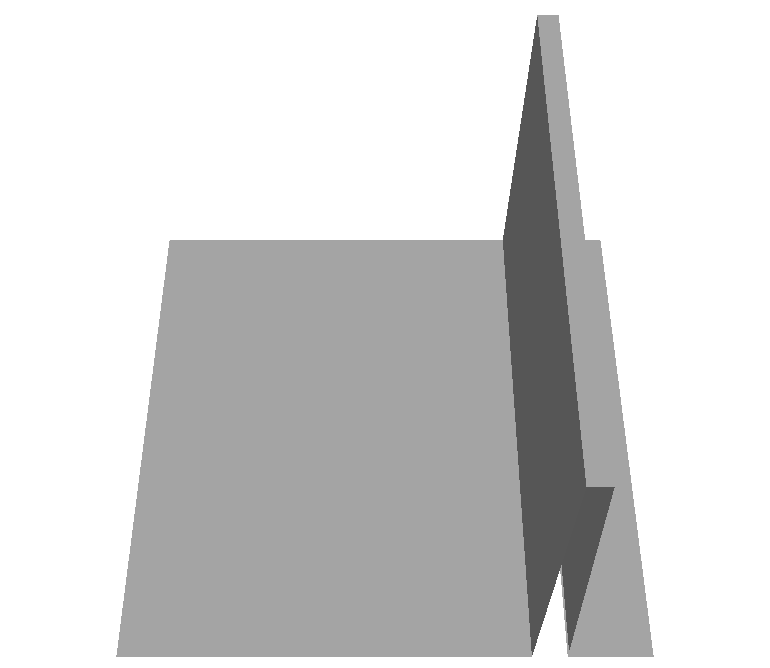
\includegraphics[width=\linewidth]{../img/5/custom_patches/walls_front/all/26-3d.png}
    \end{subfigure}
    \begin{subfigure}[b]{0.065\textwidth}
    
\includegraphics[width=\linewidth]{../img/5/custom_patches/walls_front/all/25-3d.png}
    \end{subfigure}
    \begin{subfigure}[b]{0.065\textwidth}
    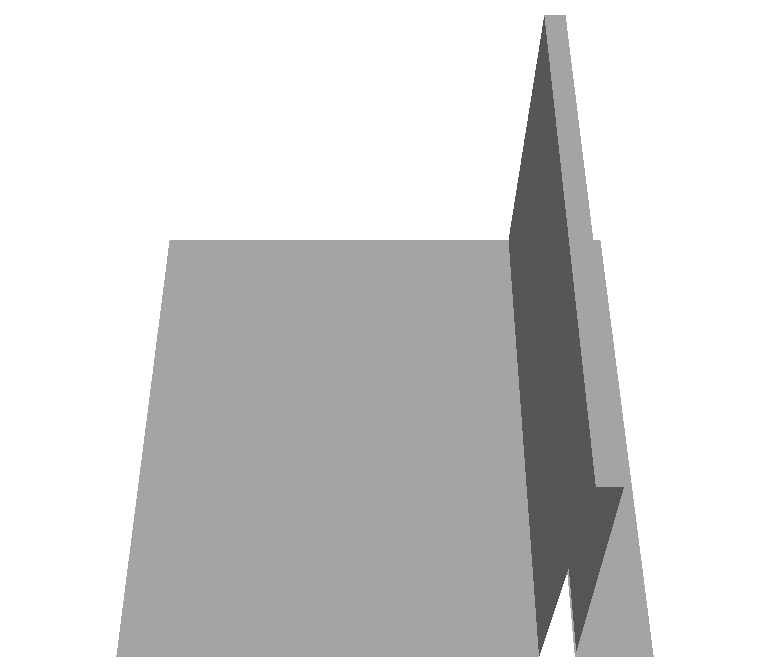
\includegraphics[width=\linewidth]{../img/5/custom_patches/walls_front/all/24-3d.png}
    \end{subfigure}
    \begin{subfigure}[b]{0.065\textwidth}
    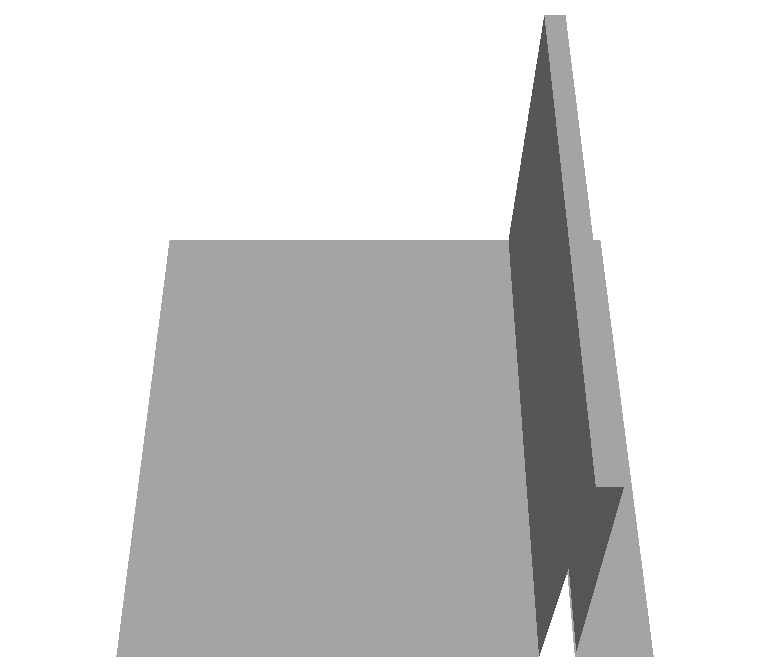
\includegraphics[width=\linewidth]{../img/5/custom_patches/walls_front/all/23-3d.png}
    \end{subfigure}
    \begin{subfigure}[b]{0.065\textwidth}
    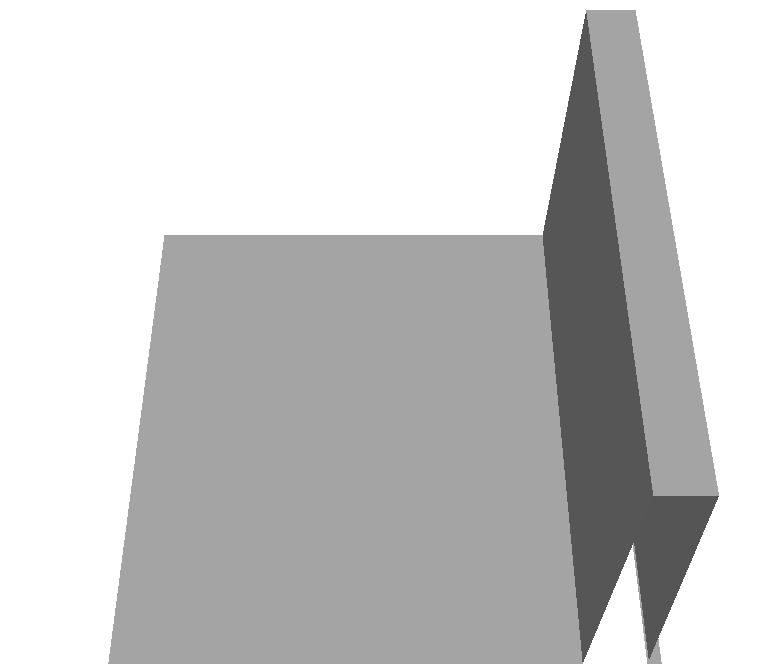
\includegraphics[width=\linewidth]{../img/5/custom_patches/walls_front/all/22-3d.png}
    \end{subfigure}
    \begin{subfigure}[b]{0.065\textwidth}
    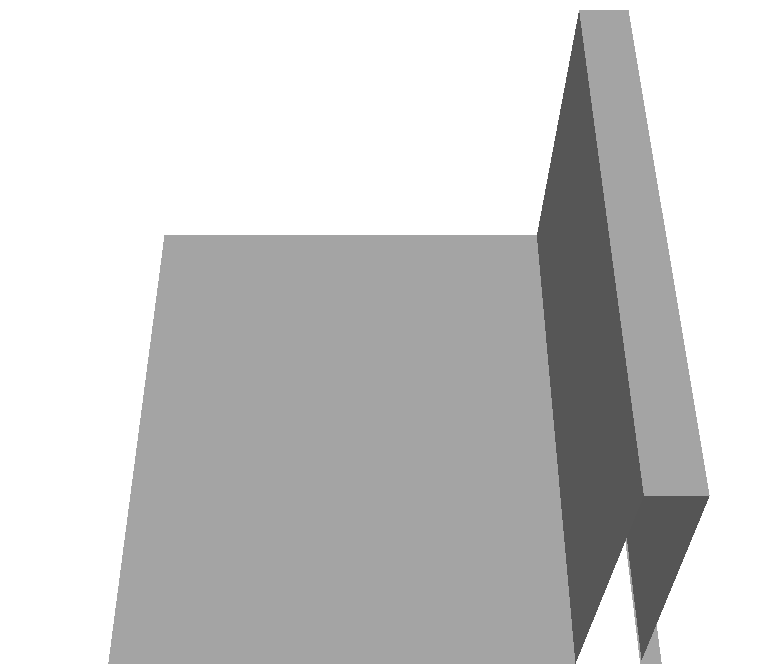
\includegraphics[width=\linewidth]{../img/5/custom_patches/walls_front/all/21-3d.png}
    \end{subfigure}
    \begin{subfigure}[b]{0.065\textwidth}
    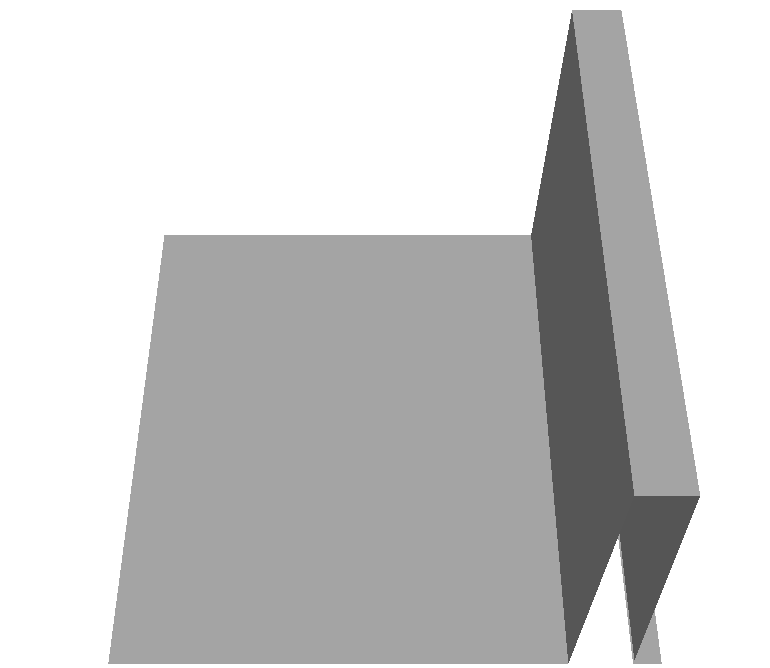
\includegraphics[width=\linewidth]{../img/5/custom_patches/walls_front/all/20-3d.png}
    \end{subfigure}
    \begin{subfigure}[b]{0.065\textwidth}
    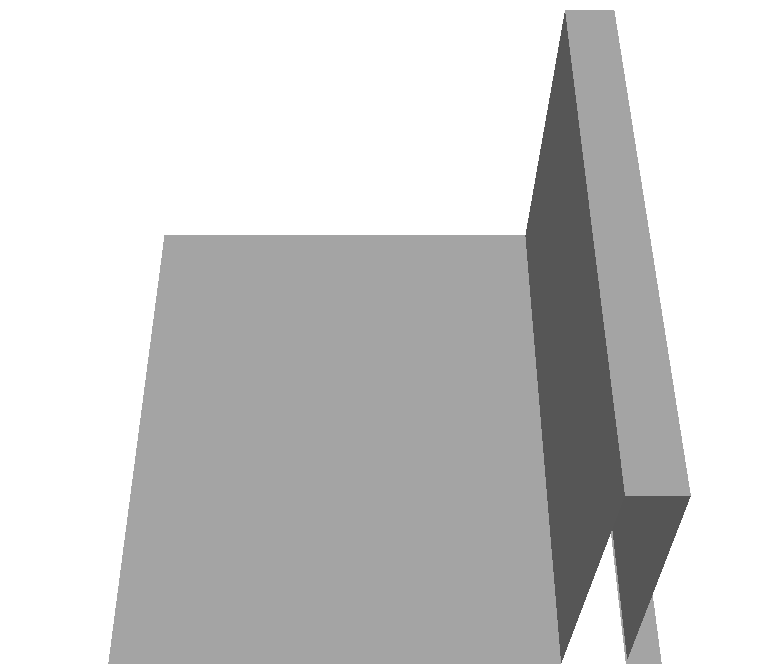
\includegraphics[width=\linewidth]{../img/5/custom_patches/walls_front/all/19-3d.png}
    \end{subfigure}
    \begin{subfigure}[b]{0.065\textwidth}
    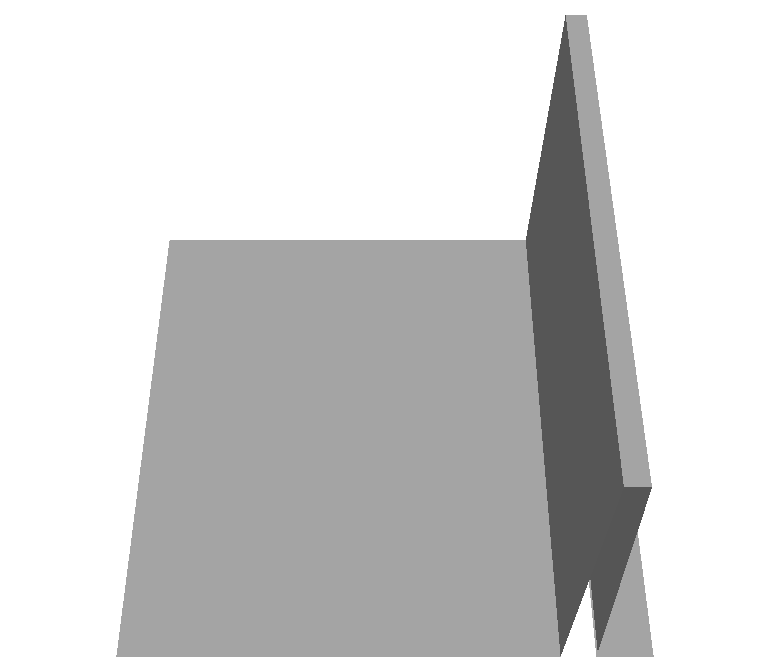
\includegraphics[width=\linewidth]{../img/5/custom_patches/walls_front/all/18-3d.png}
    \end{subfigure}
    \begin{subfigure}[b]{0.065\textwidth}
    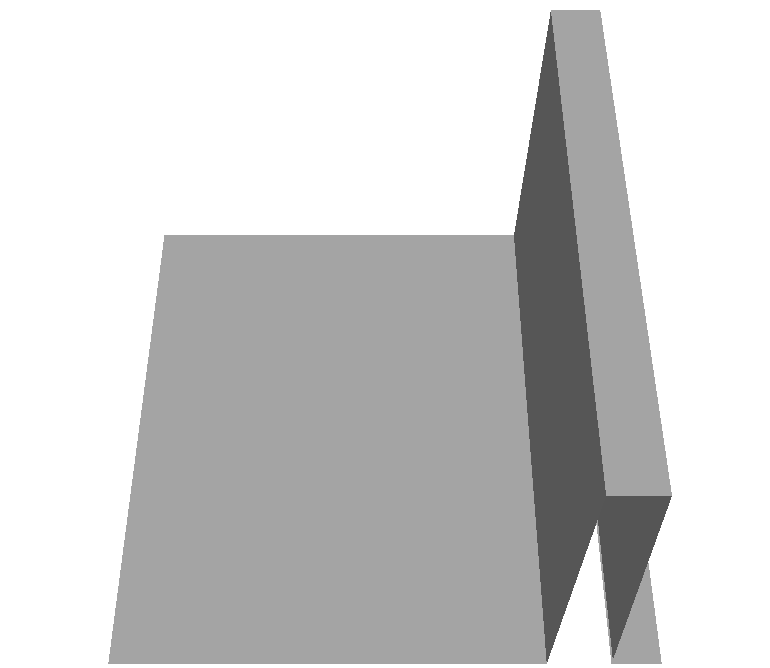
\includegraphics[width=\linewidth]{../img/5/custom_patches/walls_front/all/17-3d.png}
    \end{subfigure}
    \begin{subfigure}[b]{0.065\textwidth}
    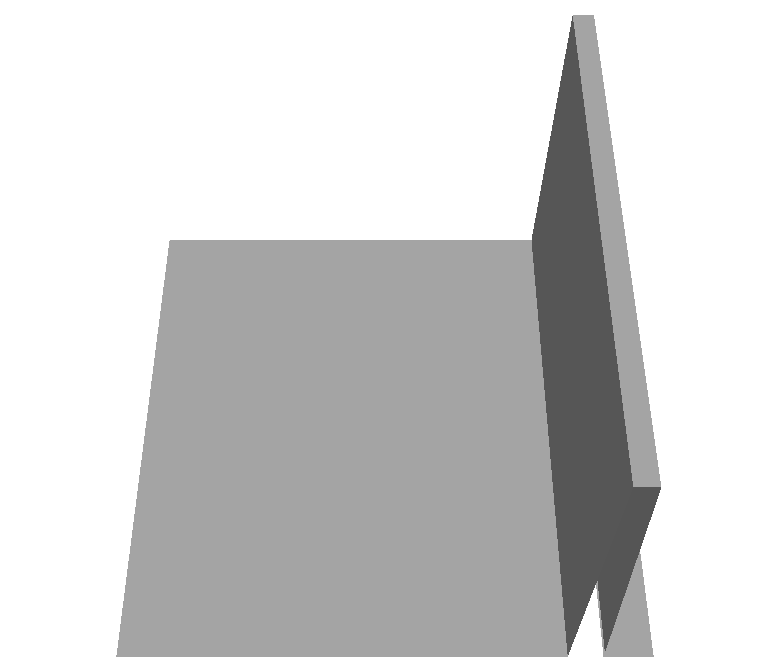
\includegraphics[width=\linewidth]{../img/5/custom_patches/walls_front/all/16-3d.png}
    \end{subfigure}
    \begin{subfigure}[b]{0.065\textwidth}
    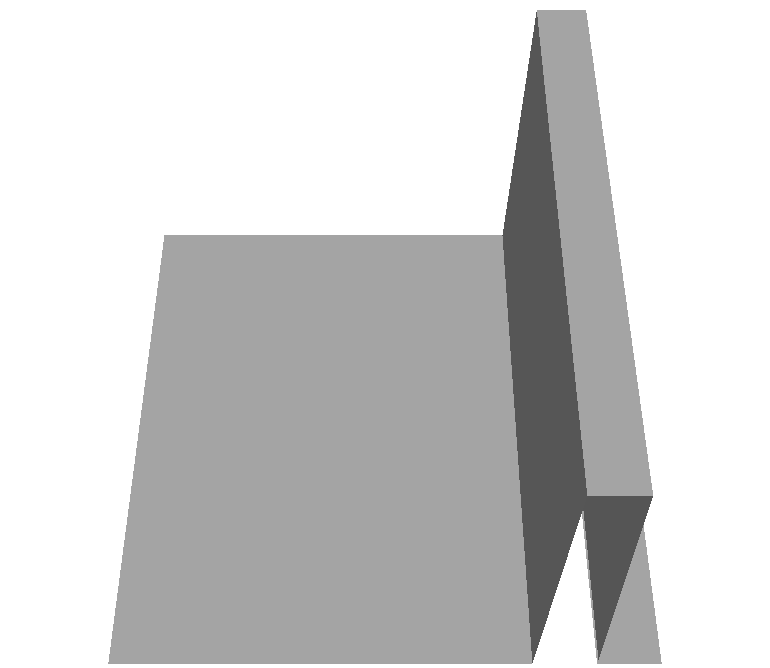
\includegraphics[width=\linewidth]{../img/5/custom_patches/walls_front/all/15-3d.png}
    \end{subfigure}
    \begin{subfigure}[b]{0.065\textwidth}
    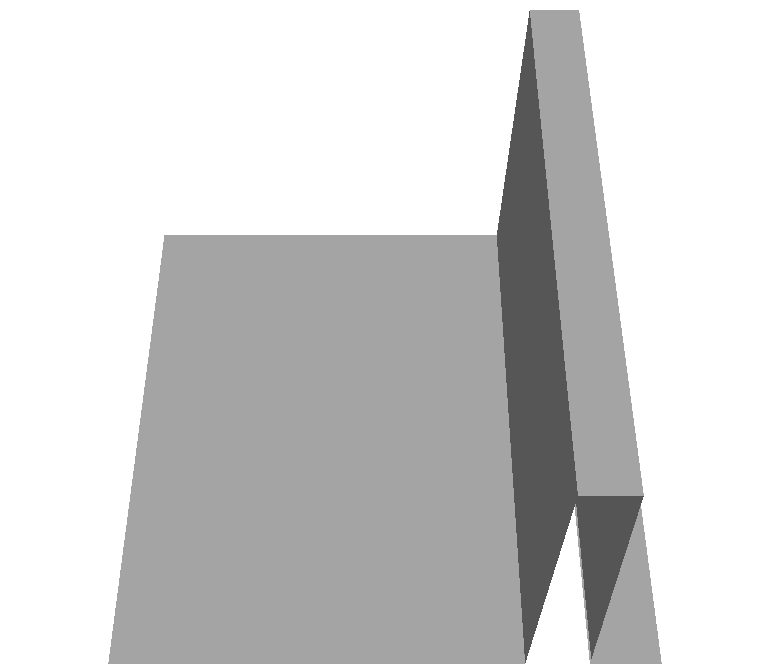
\includegraphics[width=\linewidth]{../img/5/custom_patches/walls_front/all/14-3d.png}
    \end{subfigure}
    \begin{subfigure}[b]{0.065\textwidth}
    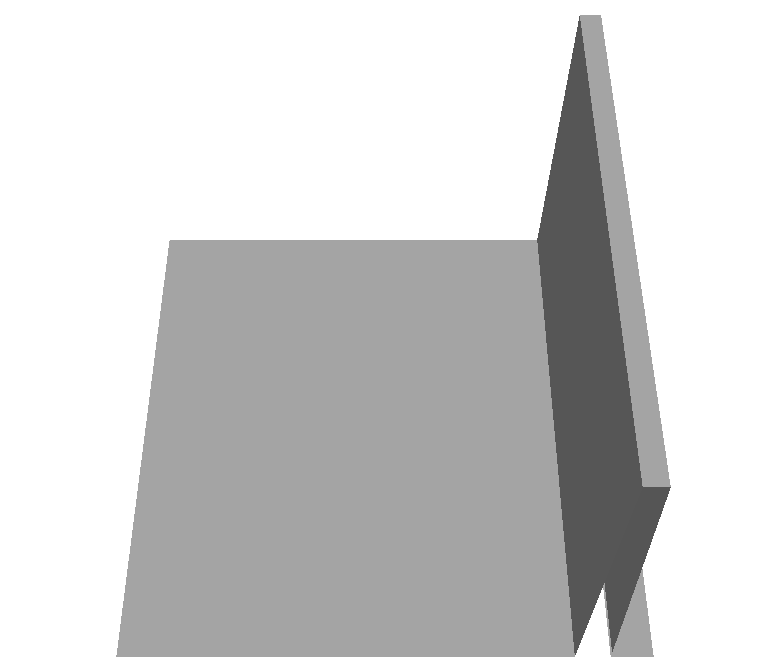
\includegraphics[width=\linewidth]{../img/5/custom_patches/walls_front/all/13-3d.png}
    \end{subfigure}
    \begin{subfigure}[b]{0.065\textwidth}
    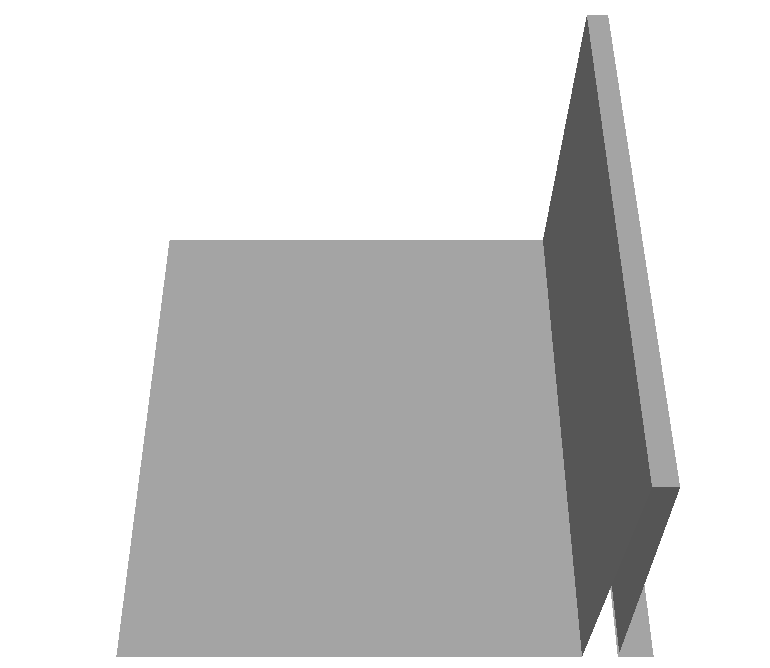
\includegraphics[width=\linewidth]{../img/5/custom_patches/walls_front/all/12-3d.png}
    \end{subfigure}
    \begin{subfigure}[b]{0.065\textwidth}
    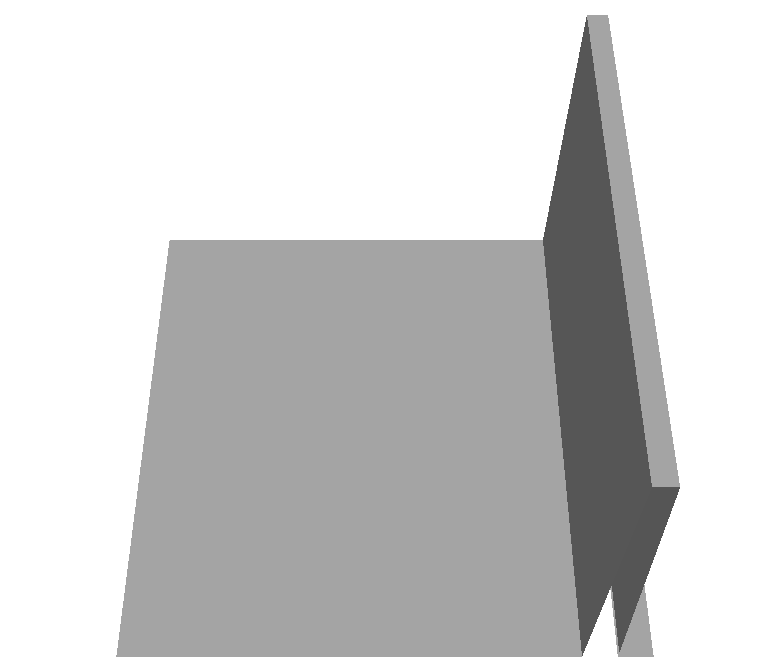
\includegraphics[width=\linewidth]{../img/5/custom_patches/walls_front/all/11-3d.png}
    \end{subfigure}
    \begin{subfigure}[b]{0.065\textwidth}
    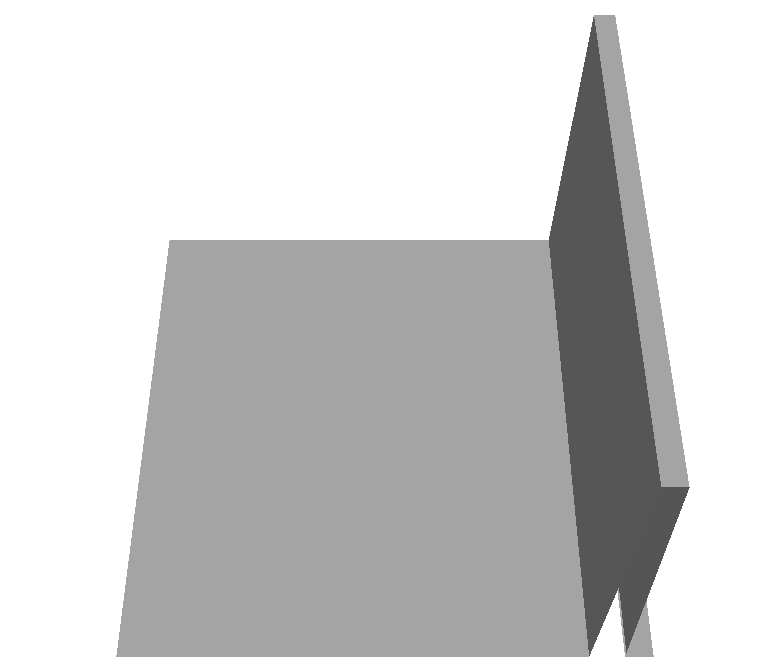
\includegraphics[width=\linewidth]{../img/5/custom_patches/walls_front/all/10-3d.png}
    \end{subfigure}
    \begin{subfigure}[b]{0.065\textwidth}
    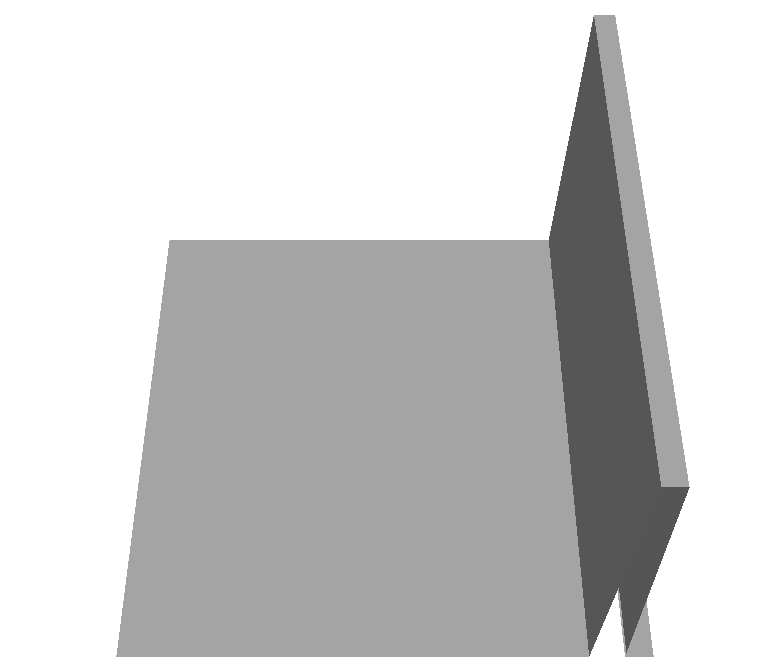
\includegraphics[width=\linewidth]{../img/5/custom_patches/walls_front/all/09-3d.png}
    \end{subfigure}
    \begin{subfigure}[b]{0.065\textwidth}
    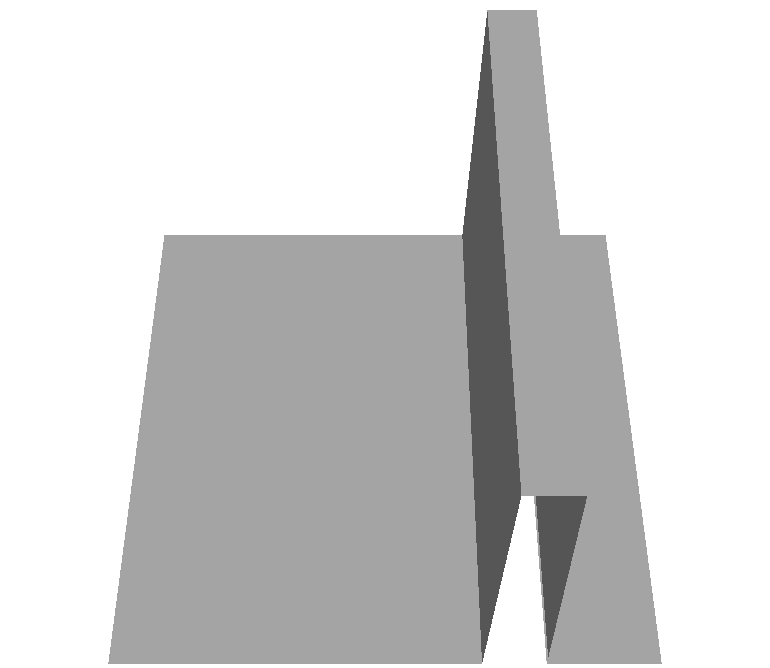
\includegraphics[width=\linewidth]{../img/5/custom_patches/walls_front/all/08-3d.png}
    \end{subfigure}
    \begin{subfigure}[b]{0.065\textwidth}
    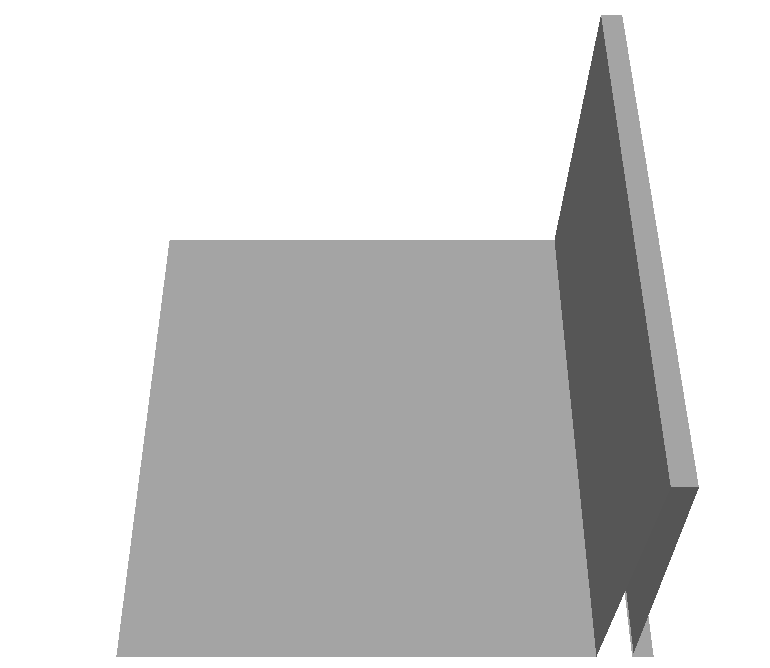
\includegraphics[width=\linewidth]{../img/5/custom_patches/walls_front/all/07-3d.png}
    \end{subfigure}
    \begin{subfigure}[b]{0.065\textwidth}
    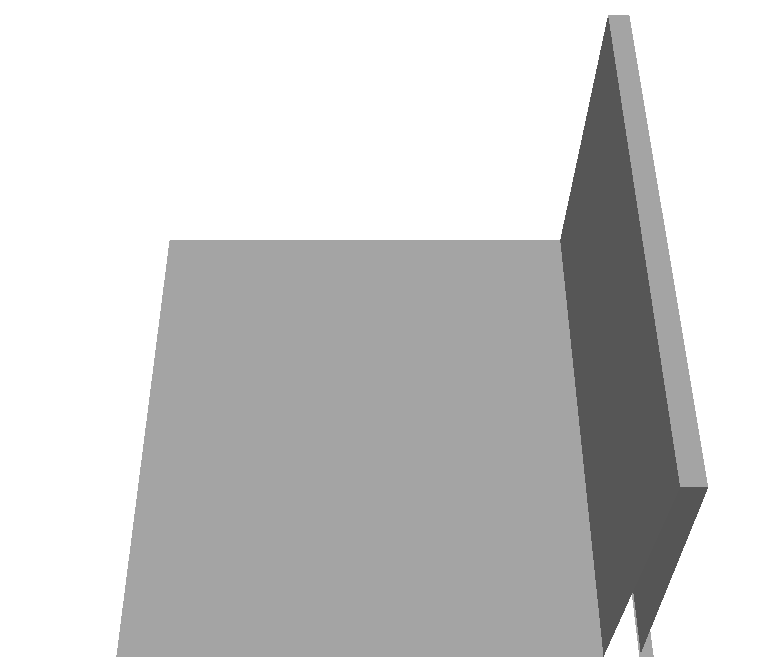
\includegraphics[width=\linewidth]{../img/5/custom_patches/walls_front/all/06-3d.png}
    \end{subfigure}
    \begin{subfigure}[b]{0.065\textwidth}
    \includegraphics[width=\linewidth]{../img/5/custom_patches/walls_front/all/05-3d.png}
    \end{subfigure}
    \begin{subfigure}[b]{0.065\textwidth}
    \includegraphics[width=\linewidth]{../img/5/custom_patches/walls_front/all/04-3d.png}
    \end{subfigure}
    \begin{subfigure}[b]{0.065\textwidth}
    \includegraphics[width=\linewidth]{../img/5/custom_patches/walls_front/all/03-3d.png}
    \end{subfigure}
    \begin{subfigure}[b]{0.065\textwidth}
    \includegraphics[width=\linewidth]{../img/5/custom_patches/walls_front/all/02-3d.png}
    \end{subfigure}
    \begin{subfigure}[b]{0.065\textwidth}
    \includegraphics[width=\linewidth]{../img/5/custom_patches/walls_front/all/01-3d.png}
    \end{subfigure}
    \begin{subfigure}[b]{0.065\textwidth}
    \includegraphics[width=\linewidth]{../img/5/custom_patches/walls_front/all/00-3d.png}
    \end{subfigure}
    \caption{Tested patches with $1$m wall at increasing distance from Krock.}
    \end{figure}

Given those inputs to the model, we get the following predictions

\begin{table}[H]
    \centering
    \begin{tabular}{l|cc}
        Distance(cm) & Prediction \\ 
        \hline
        0 - 19  & Not traversable \\ 
        19 - end & Traversable \\ 
        \hline
    \end{tabular}
    \caption{Model prediction from the wall patches}
\end{table}
To be sure the results are correct, we run the last non traversable patch and the first traversable
on the simulator to get the real advancement. In the simulator, Krock advances $19.9$cm on the non traversable patch $(a)$ where the wall is at distance of $19.6$cm from the head. While, on the first traversable where the wall is at a distance of $20.5$cm, the robot was able to travel for $22.4$. This shows that the model was able to correctly understand that, in this case, the distance of the obstacle is the more relevant than its height.
\begin{figure}[H]
    \centering
    \begin{subfigure}[b]{0.33\textwidth}
        \includegraphics[width=\linewidth]{../img/5/custom_patches/walls_front/1-2d.png}
        \end{subfigure}   
    \begin{subfigure}[b]{0.33\textwidth}
        \includegraphics[width=\linewidth]{../img/5/custom_patches/walls_front/2-2d.png}
    \end{subfigure}   \\
    \begin{subfigure}[b]{0.33\textwidth}
        \includegraphics[width=\linewidth]{../img/5/custom_patches/walls_front/1-3d.png}
        \caption{Distance  $19.6$cm}
    \end{subfigure}   
    \begin{subfigure}[b]{0.33\textwidth}
        \includegraphics[width=\linewidth]{../img/5/custom_patches/walls_front/1-3d.png}
        \caption{Distance $20.5$cm}
    \end{subfigure}   
\end{figure}
Due to the patch resolution and some luck, the robot may advance more than the distance between its head and the wall. 

\end{document}